\documentclass[__main__.tex]{subfiles}

\begin{document}

\section{Спектральный признак устойчивости в явной разностной схеме (шаблон -- "крест") для одномерного гиперболического уравнения}

Рассмотрим задачу Коши:

\begin{equation} \label{34.1}
\begin{cases}
\frac{\partial^2 U}{\partial t^2} - \frac{\partial^2 U}{\partial x^2} = 0, \ \left(x,t\right) \in \mathbb{R} \times \left(0,T\right) \\
U \left(x,0\right) = \varphi \left(x\right), \ \frac{\partial U}{\partial t} \left(x,0\right) = \psi \left(x\right), \ x\in \mathbb{R}
\end{cases}
\end{equation}


Конечно-разностную схему рассмотрим на сетке:

$$
C = A \times B = \langle \left(x_k, t^n\right) = \left(k h; n t\right): k \in \mathbb{Z}, n = \overline{0,N} \rangle
$$

Конечно-разностный аналог, аппроксимирующий задачу \ref{34.1}, создаётся с помощью $C$ - сеточной функции; заданный на слое n времени в виде: $U^n_{\left(\cdot\right)} = \left(U^n_k \in\mathbb{R}\right)_{\mathbb{Z}}$ в виде (явная схема):

\begin{figure}[ht]
	\centering
	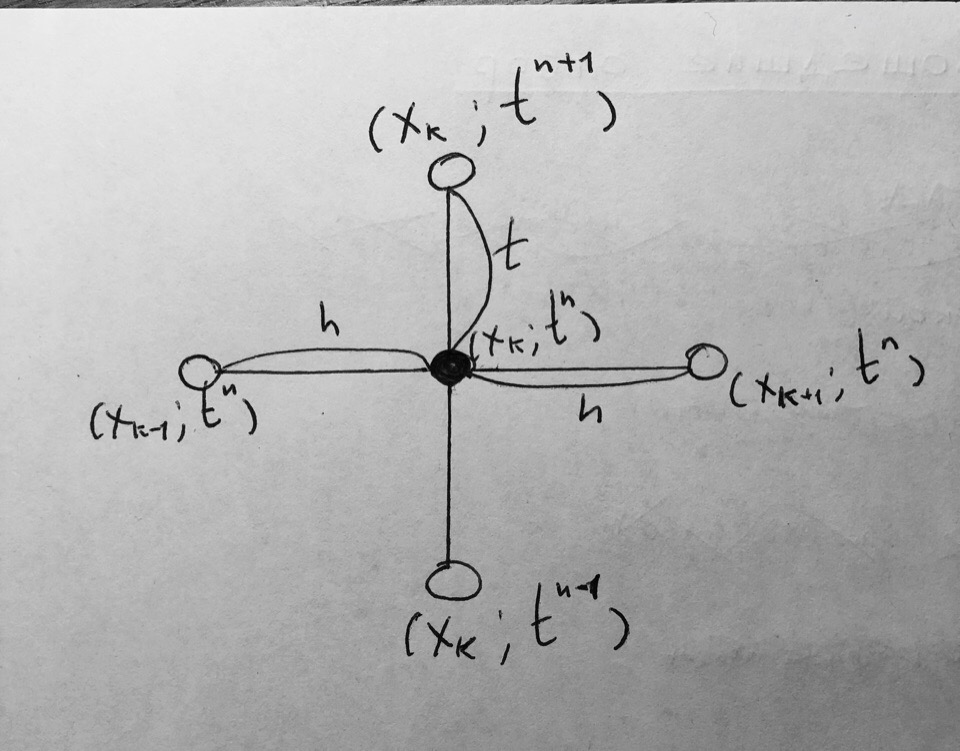
\includegraphics[width=0.4\linewidth]{img/img_34-1}
	\caption{}
	\label{img_34.1}
\end{figure}

\begin{equation}\label{34.2}
\begin{cases}
\frac{U^{n+1}_k - 2U^n_k+U^{n-1}_k}{t^2} - \frac{U^n_{k+1} -2U^n_k+U^n_{k-1}}{h^2} = 0 \\
U^0_k = \varphi_k, \ \frac{U^1_k - U^0_k}{t} \psi_k, \ k\in\mathbb{Z}, \ n = \overline{1,N-1}
\end{cases}
\end{equation}

\paragraph{Спектралный признак}

$U^{n-1}_k = e^{i \alpha k}$, $U^n_k = \lambda\left(\alpha\right) \cdot e^{i \alpha k}$, $U^{n+1}_k = \lambda^2 \left(\alpha\right) e^{i \alpha k}$.

Из \ref{34.2} получаем:

\begin{equation}
\begin{cases}
\frac{e^{i\alpha k} \left(\lambda^2 - 2 \lambda + 1\right)}{t^2} - \lambda \frac{e^{i \alpha k} \left(e^{i\alpha} - 2 + e^{-i\alpha}\right)}{h^2} = 0 \\
\text{\ae} = \frac{t}{h} - \text{параметр Куранта}
\end{cases}
\end{equation}

$$
\lambda^2 - 2 \lambda + 1 - \text{\ae}^2 \lambda \left(e^{i\alpha - 2 + e^{-i \alpha}}\right) = 0
$$

$$
\lambda^2 - 2 \lambda \left( 1 - 2\text{\ae}^2 \sin^2 \frac{\alpha}{2} \right) + 1 = 0
$$

$$
D = 4 \text{\ae}^2 \sin^2 \frac{\alpha}{2} \left(\text{\ae}^2 \sin^2 \frac{\alpha}{2} - 1 \right)
$$

\begin{enumerate}
	\item 
	$$
	\text{\ae}^2 \sin^2 \frac{\alpha}{2} - 1 \leq 0, \ \alpha \in [0;2\pi] \Rightarrow \text{\ae}^2 - 1 \leq 0 \Rightarrow \frac{t}{h} = \text{\ae} \leq 1 \Rightarrow \text{устойчива}
	$$
	
	\item 
	$$
	\text{\ae}^2 - 1 > 0, \Rightarrow \frac{t}{h} = \text{\ae} > 1 \Rightarrow max \{ \left|\lambda \left(\alpha\right)\right|: \alpha \in[o;2\pi] \} > 1 \Rightarrow \text{неустойчива}
	$$
\end{enumerate}
\end{document}